\documentclass[11pt,a4paper]{article}
\usepackage[utf8]{inputenc}
\usepackage[english]{babel}

% Citations and bibliography
\usepackage{natbib}
\bibliographystyle{abbrvnat}

% Graphics
\usepackage{xcolor}
\usepackage{graphicx}
\graphicspath{{Figures/}}

% Custom commands
\newcommand{\silvan}[1]{\textcolor{blue}{[#1]}}

% Math
\usepackage{amssymb}
\usepackage{mathtools}
% Relations between variables
\DeclareMathOperator*{\CI}{{\,\perp\mkern-12mu\perp\,}}
\DeclareMathOperator*{\nCI}{{\,\not\mkern-1mu\perp\mkern-12mu\perp\,}}
\DeclareMathOperator*{\SEP}{\perp}
\DeclareMathOperator*{\nSEP}{\not\perp}
\newcommand{\indep}[4]{{#1} \CI_{#4} {#2} \given {#3}}
\newcommand\dep[4]{{#1} \nCI_{#4} {#2} \given {#3}}
\newcommand\sep[4]{{#1} \SEP_{#4} {#2} \given {#3}}
\newcommand\con[4]{{#1} \nSEP_{#4} {#2} \given {#3}}
\newcommand{\dsep}[4]{{#1} \SEP_{#4}^d {#2} \given {#3}}
\newcommand{\dcon}[4]{{#1} \nSEP_{#4}^d {#2} \given {#3}}
\newcommand{\sigmasep}[4]{{#1} \SEP_{#4}^\sigma {#2} \given {#3}}
\newcommand{\sigmacon}[4]{{#1} \nSEP_{#4}^\sigma {#2} \given {#3}}
\newcommand{\Prb}{\mathbb{P}}
\newcommand{\marg}[1]{\mathrm{marg}_{#1}}
\newcommand{\intervene}{\mathrm{do}}
% Arrows (oriented, star, circle)
\newcommand{\ot}{\leftarrow}
\newcommand{\oto}{\leftrightarrow}
\newcommand{\ots}{\leftarrow\mkern-13mu\ast\,}
\newcommand{\otc}{\leftarrow\mkern-9mu\circ\,}
\newcommand{\sto}{\,\ast\mkern-13mu\to}
\newcommand{\stt}{\,\ast\mkern-13mu\relbar\!\!\!\relbar}
\newcommand{\tts}{\relbar\!\!\!\relbar\mkern-13mu\ast\,}
\newcommand{\sts}{\,\ast\mkern-10mu\relbar\mkern-10mu\ast\,}
\newcommand{\ctc}{\,\circ\mkern-9mu\relbar\mkern-9mu\circ\,}
\newcommand{\cto}{\,\circ\mkern-9mu\rightarrow}
% Other
\newcommand\given{\,|\,}

\title{Causal Analysis and Gene Expression Data}

\author{Silvan de Boer \\
  {\tt silvandeboer@gmail.com}}

\date{}

\begin{document}
% \twocolumn
\maketitle

% % \section*{Introduction}

% % \section*{Background}
SCMs
Cycles, latent confounding, selection bias, interventions, constraint VS score-based, faithfulness, causal sufficiency (Markov properties), graph types, evt. independence oracle (Chickering et al., 2004? [according to \citeauthor{claassen2013learning}])

\section*{Related Work}

% First short summary, 
% then in detail per paper (Historical context/storyline)

% Data types: observational, interventional, fixed variables

% \textbf{Factors}
% \begin{itemize}
%     \item Confounding
%     \item Mechanism function
%     \item Cycles
%     \item Intervention: perfect, stochastic, mechanism change, activity intervention, other
%     \item Known intervention targets
%     \item Taks/Output: global causal discovery (MAG/MG?, strength of links?), ancestral relations, predict expression after intervention, ...
%     \item Fixed variables
%     \item Computation time
% \end{itemize}


% \textbf{Papers}
% \begin{itemize}
%     \item [\cite{yang2018characterizing}] 
%         Generalize \cite{hauser2012characterization} from perfect to general interventions. Define interventional Markov equivalence class, which is identified from general intervention experiments. First provably consistent algotithm for learning DAGs. Simulated and biological datasets, with observational and intervention data.
%     \item [\cite{mooij2013cyclic}]
%         Observational and interventional equilibrium data (cytometry \cite{sachs2005causal}). Deals with feedback loops and continuous data. Model activity (how the equilibrium distributions of direct effects is influenced) instead of abundance of compounds, so standard intervention formalism of \citet{pearl2009causality} is not applicable. Nonlinear mechanisms are approximated by coupled local linearizations. 
%     \item [\cite{hauser2012characterization}]
%         Every interventional Markov equivalence class can be represented by an interventional essential graph (like CPDAG in obs. case). Generalize GES to the Greedy Interventional Equivalence Search algorithm (GIES). Tested in simulation study.
%     \item [\cite{tian2001causal}]
%         Possibly infer some environmental change?
%     \item [\cite{forre2018constraint}]
%         Introduces modelling framework of modular SCMs (mSCM) and $\sigma$-connection graphs, extending $\sigma$-separation to work on them. ASD (Accounting for Strong Dependences; score-based) method tested on synthetic data and solved with an ASP (Answer Set Programming) solver. Very computationally expensive.
%     \item [\cite{versteeg2019boosting}]
%         Estimates of LCD and ICP following JCI framework. 
% \end{itemize}


% \textbf{Datasets}
% \begin{itemize}
%     \item [\cite{kemmeren2014large}]
%         Gene expression dataset.
%     \item [\cite{sachs2005causal}] 
%         Flow cytometry in human immune system cells; signalling network; compare to consensus network
% \end{itemize}

% \textbf{Methods}

\subsection*{Constraint-Based Causal Discovery}
Constraint-based approaches derive constraints from the data, and use it to restrict the class of possible underlying causal graphs. Causal inference is treated as a constraint-satisfaction problem. Generally, conditional independence relations (CIR) are chosen as constraints, which can be used to derive the separation of variables and the orientation of edges in the graph. Some prominent methods are described below.

\textbf{Inductive Causation} (IC) was introduced by \citet{verma1991equivalence} and generally describes how we can induce a PDAG from conditional independences in the data. The algorithm consists of two steps: inducing the skeleton and orienting the edges. For every pair of variables $a$ and $b$, we check whether there is an edge in the PDAG. Using the faithfulness assumption, we add an edge if there is no separating set of variables $S_{ab}$ that makes $a$ and $b$ conditionally independent ($\nexists S : \indep{a}{b}{S_{ab}}{}$). One easy step of edge orientation uses the separation criterion of colliders. If two non-adjacent variables $a$ and $b$ share a neighbour $c$ that is not in $S_{ab}$, it must be a collider on the path and we induce edge orientation $a\to c \ot b$. Application of additional orientation rules lead us to a maximally oriented PDAG, which describes the Markov equivalence class of all causal graphs that induce the joint data distribution. One early set of such rules was described by \citet{spirtes2000causation} in the SGS algorithm, which was named after the authors.
            
IC is quite limited, because it relies on several assumptions about the underlying SCM (e.g. causal sufficiency), and its naive implementation is costly due to the search over all separating sets $S_{ab}$.

\textbf{PC}, named after its inventers Peter Spirtes and Clark Glymour \citep{spirtes1991algorithm}, reduces the cost of naive IC. A systematic algorithm finds the separating sets $S_{ab}$ in polynomial time. Starting from a fully-connected graph, edges are systematically removed by considering separating sets of increasing cardinality, and only taking into account the variables that neighbour $a$ and $b$. For example, first edges are removed between variable pairs that are independent given the empty set (cardinality 0). Then, edges are removed between remaining adjacent variable pairs that are independent given one of their neighbours. Already some possible separating sets can be skipped here, because edges were removed in the previous step. Therefore, as we consider larger possible separating sets, the number of neighbours to choose from decreases.
            
\textbf{Fast Causal Inference} (FCI) extends PC to allow for selection bias and latent confounding. Dropping the causal sufficiency assumption, means that it should consider some possible separating sets $S_{ab}$ that contain variables not adjacent to $a$ or $b$ (specifically, their ancestors). FCI is a feasible algorithm for datasets with many variables when the underlying graph is sparse and bidirected edges are not too much chained together. It was first introduced by \citet{spirtes1999algorithm}, and gradually developed since then. A modern version named FCI+ by \citet{claassen2013learning} is relatively fast. It finds the complete PAG in polynomial time.
            
\textbf{Invariant Causal Prediction} (ICP) does not infer a complete equivalence class of causal graphs from the data, but is concerned with local features of that graph. In its original formulation by \citet{peters2016causal} it outputs a subset of parents of a target variable, and in a later adaptation by \citet{mooij2016joint} the output is a subset of ancestors. In comparison to the previous methods, this approach uses data from different contexts.

When we model the context (e.g. intervention) as a variable that is not a cause of the target variable, then the conditional distribution of the target variable given its direct causes is invariant to the value of the context variable. This property is used by ICP to find parent or ancestor relations in data from different contexts. 

In a naive implementation, we would have to investigate every possible parent set for every target variable, making the complexity exponential in the number of variables. Since (direct) causes tend to correlate with their effect, it is reasonable to only consider variables that have a relatively high correlation with the target variable. Such an approximation was used by \citet{peters2016causal} and \citet{meinshausen2016methods} to apply ICP to the dataset of \citet{kemmeren2014large} with over six thousand variables.

\textbf{Local Causal Discovery} (LCD) is a simple local method that looks at ancestral causal relations in the context of a changing environment. In the data, we marginalize over three variables ($C, X, Y$), one of which is exogenous ($C$). This means that we have the domain knowledge that this variable is not a direct or indirect effect of any endogenous variables. Next, we perform three statistical tests: $\indep{C}{Y}{X}{}$, $C \nCI X$ and $X \nCI Y$. If these tests are positive, \citep{cooper1997simple} proves that there is a relationship $X \to Y$. 

This method allows for latent confounders, and assumes that there is no selection bias. Note that this method can find only a limited subset of ancestral relations. \citep{cooper1997simple} prove the theory by listing all possible causal graphs of three variables in which the context variable is not caused by endogenous variables. They note that of the 32 networks in which $X$ causes $Y$, LCD is only able to identify this relation in 3 cases. The others are not identified, because there are other configurations that induce the same independence relations. For example, if $C$ causes $Y$ not only through $X$, but via another path as well, we will not find that $X$ causes $Y$.  

% e.g. Trigger?\citep{chen2007harnessing}. Local strategy.

\textbf{Y-structures} are a pattern in a Partial Ancestral Graph (PAG), which has information about ancestral relations between four random variables. \citet{mooij2015empirical} showed that a set of independence tests can be used to infer some ancestral relations from observational data. This local method can be used to find an incomplete set of ancestral relations in the underlying SCM. 

Specifically, we marginalize over four random variables $X$, $Y$, $Z$ and $U$. Then we perform four statistical tests: $\indep{Z}{Y}{X}{}$, $Z \nCI Y$, $\dep{Z}{U}{X}{}$ and $Z \CI U$. If all tests are positive, there are only two possible PAGs representing the marginalization over the four variables, which are called Y-structure (a term coined for a score-based method by \citet{mani2006bayesian}) and Extended Y-structure. In both PAGs, we can use the backdoor criterion to infer that $p(Y\given \intervene(X=x))=p(Y\given X)$.

\citet{mooij2015empirical} investigate the performance effect of adding more independence tests. By adding two more tests, the Y-structure remains the only possible PAG. After that, more redundant independence tests can be added. Adding more tests necessarily reduces recall, but precision can improve if the extra tests eliminate false positives. Interestingly, in their experiments on synthetic data, maximum precision is not always achieved with the minimum or maximum number of tests.

An interesting insight from \citet{mooij2015empirical} is that the faithfulness assumption becomes more problematic as the number of random variables grows. The data is sampled from a SCM, which makes the faithfulness assumption very reasonable. However, it appears that the marginalized data can be almost faithless to the supposed PAG. 

% Mooij2015empirical: Our  findings  illustrate  that  violations of strong faithfulness become increasinglylikely  in  the  presence  of  many  latent  variables,and  this  can  significantly  deterioriate  the  accu-racy of constraint-based causal prediction algo-rithms that assume faithfulness.


    
\subsection*{Score-Based Causal Discovery}
Score-based approaches search for the causal graph that optimizes some loss function, often based on independences in the data. Some methods are discussed below.
% (e.g., Cooper and Herskovits,1992; Heckerman et al., 1995; Chickering, 2002; Koivisto and Sood, 2004) (see: Peters 7.2)
% Mani et al 2006: disadvantages of constraint-based (citing Heckerman et al., 1999): (1) the inability to include prior belief in the form of structure probabilities, (2) the output is based on the significance level used for the independence tests, and (3) there is no quantification of the strength of the hypothesis that is output.

\textbf{Accounting for Strong Dependences} (ASD) is a method that focusses on graphs satisfying dependences in the data, whereas most methods focus on the independences. The groundwork of the method was layed by \citet{hyttinen2014constraint}. Dependence and independence relations in the data are encoded as soft constraints in ASP (Answer Set Programming), together with rules that determine that the solution should be a valid graph. The solution is then found by an ASP solver, that minimizes the loss computed as the sum of the weights of the constraints that are not satisfied. This method can only be applied to problems with a small number of variables, because the number of dependence and independence relations quickly becomes very large.

\citet{magliacane2016ancestral} compute weights based on the p-value of the conditional independence test and the significance level, such that strong dependences obtain a larger weight than independences. They also provide a method to compute a confidence score for single features of the graph (like an ancestral relation) by solving two optimization problems and subtracting the losses. In one problem, the presence of the feature is added as a hard constraint, in the other the absence is added as a hard constraint. 

As part of their Joint Causal Inference (JCI) framework, \citet{mooij2016joint} adapt the ASD method to include interventional data. They simply add some constraints to the ASP problem that encode their JCI assumptions for interventional data.


% Here we introduce a novel JCI implementation that builds on the algorithm by Hyttinenet al. (2014) and its generalization toσ-separation (Forr ́e and Mooij, 2018) and some of theextensions proposed by Magliacane et al. (2016b
% \item [\cite{forre2018constraint}]
%         Introduces modelling framework of modular SCMs (mSCM) and $\sigma$-connection graphs, extending $\sigma$-separation to work on them. ASD (Accounting for Strong Dependences; score-based) method tested on synthetic data and solved with an ASP (Answer Set Programming) solver. Very computationally expensive.

\textbf{Greedy Equivalence Search} (GES) was first introduced by \citet{meek1997graphical} and further detailed by \citet{chickering2002optimal}. A search for the Markov equivalence class (MEC) is performed in two phases. Our graph is initialized without edges. In the first phase, we move between MECs by adding edges. In each step, we consider the set of MECs that are one edge addition away from the current MEC. Reversing a covered edge does not change the MEC, so we need to consider every combination of covered edge reversals, followed by a single edge addition, followed by covered edge reversals. We score the MECs and move to the one with the highest score. \citet{meek1997graphical} proposed the Bayesian scoring criterion to score DAGs in a MEC. Under some conditions this can be approximated by the Bayesian information criterion (BIC). 

Once we reach a local maximum, \citet{chickering2002optimal} shows that the MEC contains the generative distribution. The second phase is analogous to the first, but this time single edges are removed. \citet{chickering2002optimal} shows that this final MEC is a perfect map of the generative distribution.

\citet{hauser2012characterization} generalize the method to datasets with interventional data (GIES). They introduce the interventional MEC as the object of the search. The algorithm is adapted by introducing the turning phase. Repeated application of the three phases leads to the interventional MEC underlying the generative distribution. They note that the space of interventional MECs is more fine-grained, meaning that this type of data leads to improved identifiability.


\subsection*{Hybrid methods}
% \textbf{Max-Min Hill-Climbing} (MMHC) (Tsamardinos et al., 2006), for example, alternates between constraint-based and score-basedupdates.

\textbf{Sparsest Permutation} (SP) is a method proposed by \citet{raskutti2018learning} that searches for the Markov equivalence class in a space of topological orderings of random variables, using observational data. The topological ordering is a permutation of variables in which ancestors precede descendents. Given an ordering and a method to infer dependence and independence relations, we can infer a DAG that satisfies causal minimality. The SP algorithm searches over these DAGs infered from all possible permutations and selects the DAG with the smallest number of edges. \citet{raskutti2018learning} show that this algorithm is consistent, which means that it finds a DAG in the correct Markov equivalence class. This consistency relies on an assumption that is weaker than faithfulness. 

\citet{solus2017consistency} propose a greedy algorithm (GSP) that increases the number of variables that can be handled from about 10 to hundreds. The only sacrifice is that a somewhat stronger assumption is required, which is still weaker than faithfulness. They introduce the DAG associahedron, a sub-polytope of the permutohedron which indicates possible directions for the depth-first search. These directions are based on the concept of covered edge. 

\citet{wang2017permutation} adapt the algorithm further to take interventional data into account (IGSP). The score is now summed over a score for each intervention distribution. This score is a weighted sum of the number of edges in the inferred graph, excluding edges into the intervened variable, and some maximum likelihood score of the interventional data given some model assumptions.



% first with consistency proof. (permutation-based without proof:  (Bouckaert, 1992; Singh and Valtorta, 1993; Teyssier and Koller, 2005). )


\subsection*{Other}
other statistical patterns in the joint distribution can be exploited too (e.g Mooij et al., 2016; Peters et al., 2017)


% TODO: IDA (Maathuis et al. 2010), MMHC, CV-Lasso regression?, CI?

% \section*{Methods}

% \section*{Experiments}

\subsection*{Data}
A biological dataset is used to evaluate the proposed methods. The DNA of a cell contains genes that are involved in many of the cell's functions. They are often responsible for the production of a protein. The first step in this process is to copy its information to a Messenger RNA (mRNA) strand. To measure how active a specific gene is, we can measure how much of its mRNA we find in the cell.

Genes interact to fulfill a plethora of cell functions. For example, the expression of one gene might up- or down-regulate the expression of some other gene. This interaction is regulated by some biochemical process. 

For a variety of reasons, it is interesting to know how genes interact precisely, that is: what the regulatory network looks like. By jointly measuring the expression of a large set of mRNA strands we obtain an mRNA profile. Collecting a set of these profiles allows us to model the joint distribution of mRNA expression and the causal relations.

Specifically, we use mRNA profiles from \citeauthor{kemmeren2014large}. They measured a profile of 6.182 genes in cells of the yeast species \textit{Saccharomyces cerevisiae} (baker's yeast). The dataset consists of 262 observational samples obtained from unaltered wild type cells, and 1.484 interventional samples obtained from mutant cells where one gene was deactivated.

Both the observational and interventional profiles are reported relatively to some average wild type profile. \citeauthor{kemmeren2014large} report that the interventional profiles are compared to a set of 428 wild type profiles. \silvan{It is unclear if the observational profiles are compared to the same set.}

There are some details of the experiments that might be of relevance in a discussion of underlying assumptions. First of all, the researchers chose to measure only a subset of about 25\% of all genes. Selection criteria included whether genes were expected to be involved in regulating other genes, and only genes were selected that do not play a vital role in keeping the cell alive (viability).

Furthermore, the profile resulting from an experiment had to pass a quality control before being admitted to the dataset. Failing this test resulted either in repeating the experiment, or excluding the mutant. Although these checks improve the quality of the data by removing some failed experiments, they might also admit some selection bias.

A final factor to consider is that  data from previous work of the same institute is included in the dataset, specifically from \citeauthor{lenstra2011specificity} and \citeauthor{van2010functional}. The authors note that they could not find any significant differences in the data. Nevertheless, this information can be seen as a context variable, and ignoring it can be an explicit modelling assumption.

\subsection*{Ground truth}

% GT figure
\begin{figure}[h]
    \centering
    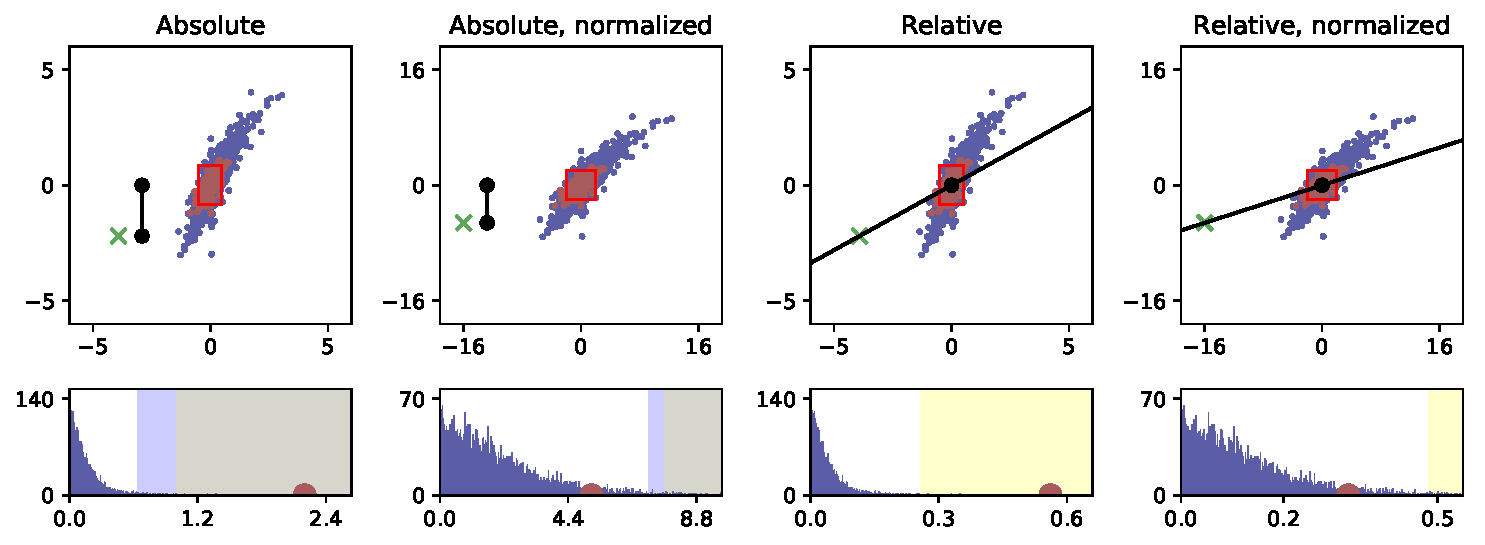
\includegraphics[width=\textwidth]{ground_truth_YHR087W_YDR074W.pdf}
    \caption{
        Different ground-truth definitions illustrated for the knock-out effects of gene YHR087W, particularly on gene YDR074W. TOP: YHR087W on the x-axis and YDR074W on the y-axis for all data points. The green cross indicates the knock-out experiment of YHR087W. The absolute ground-truth is the length of the black line segment, the relative ground-truth is the slope of the black line. The red square indicates a block of 2 standard-deviations in the observed data (red). BOTTOM: distribution of ground-truth scores of all genes in the knock-out experiment of YHR087W. The red half-circle indicates the score of gene YDR074W. The blue plane shows the 99 percentile threshold based on all data, the yellow plane shows it based only on the data from this knock-out experiment. The overlap of both planes is grey.
    }
    \label{fig:ground-truth}
\end{figure}


Value and slope, absolute and 'normalized'

Train-test splits
5-fold cross-validation; separate test set?

\subsection*{Simple analysis}
Visualisation of gene VS gene
Cycles and latent confounders

% \section*{Results}

% \section*{Analysis}

% \section*{Conclusion}

\bibliography{references}


\end{document}
